\documentclass[a4paper,11pt]{article}

% Identificação
\newcommand{\pbtitulo}{Práticas com Arduino}
\newcommand{\pbversao}{1.0}

\usepackage{../sty/tutorial}

%----------------------------------------------------------------------
% Início do Documento
%----------------------------------------------------------------------
\begin{document}

\maketitle % mostrar o título
\thispagestyle{fancy} % habilitar o cabeçalho/rodapé das páginas

%-----------------------------------------------------------------------------
% RESUMO DO ARTIGO
%-----------------------------------------------------------------------------

\begin{abstract}
\initial{A}\textbf{rduino é uma placa com microcontrolador de baixo custo e alto desempenho que se destaca por seu preço reduzido e por oferecer uma alternativa acessível para projetos de hardware personalizados.}
\end{abstract}

%-----------------------------------------------------------------------------
% CONTEÚDO DO ARTIGO
%-----------------------------------------------------------------------------
\section{Introdução}
Iremos mergulhar no mundo do Arduino e explorar projetos divertidos e amigáveis para iniciantes. Nesta entramos em sensores populares e projetos criativos que podemos construir e aprimorar o conhecimento. Essas ideias ajuda a compreender conceitos fundamentais, praticar habilidades de programação e ganhar experiência prática com eletrônica.

\textbf{ATENÇÃO} - Como usaremos ligações elétricas, esses projetos NÃO devem ser realizados por crianças sem o acompanhamento dos pais ou adulto responsável.

\section{Projetos para a prática}
Aprender a programar com Arduino por meio de exemplos práticos traz vantagens significativas, especialmente para aqueles que estão começando e deseja ver resultados rápidos. Assim não espere aqui histórias, diagramas de explicação dos componentes ou da programação, o \textbf{Leitor} desta, já deve dominar esta parte.

\textbf{Projetos práticos} favorecem a autonomia e a capacidade de resolver problemas. Ao enfrentar erros de montagem, falhas no código ou resultados inesperados, o estudante aprende a depurar, testar hipóteses e buscar soluções de forma ativa. Diferentemente do modelo tradicional, que muitas vezes é passivo e centrado na repetição de exercícios, o aprendizado com Arduíno incentiva a investigação, a criatividade e a aplicação do conhecimento em situações do cotidiano, como automação residencial, robótica e monitoramento ambiental.

Essa metodologia prepara melhor para o mercado de trabalho e para desafios tecnológicos atuais. Projetos práticos desenvolvem competências como planejamento, documentação e pensamento crítico - habilidades que vão além do conteúdo técnico. Assim, aprender Arduíno por meio de projetos não apenas torna o processo mais motivador, como também oferece uma vantagem clara em relação ao ensino tradicional, ao formar alunos mais engajados, competentes e prontos para criar soluções inovadoras.

\textbf{ATENÇÃO}: Em todos os projetos descritos utilizaremos uma placa de prototipagem (caso necessário para melhor montagem), \textit{jumpers} - fios para conexão (quantidade conforme vista no diagrama dos projetos) e o Arduino Uno (outro modelo pode ser utilizado com as devidas modificações no projeto) já configurado e iniciado para aceitar a programação C++ (veja diversos tutoriais e vídeos na Internet que ensinam como realizar este processo), que não serão descritos nos materiais necessários.

\subsection{Projeto 1 - Sensor de Presença}
Um módulo relé atua como um interruptor eletrônico, permitindo que o Arduino (que opera em baixa tensão) controle um dispositivo elétrico de alta tensão (110V/220V).

\textbf{Aviso de Segurança}: Ao trabalhar com módulos relé e lâmpadas ligadas à rede elétrica (110V ou 220V), tome extremo cuidado. Certifique-se de que tudo esteja isolado e desligado da tomada durante a montagem para evitar choques elétricos.

Este projeto possui os seguintes materiais: \vspace{-1em}
\begin{itemize}
	\item Módulo Sensor PIR
	\item Lâmpada com seu conector
	\item Módulo Relay
\end{itemize}

\begin{figure}[H]
	\centering
	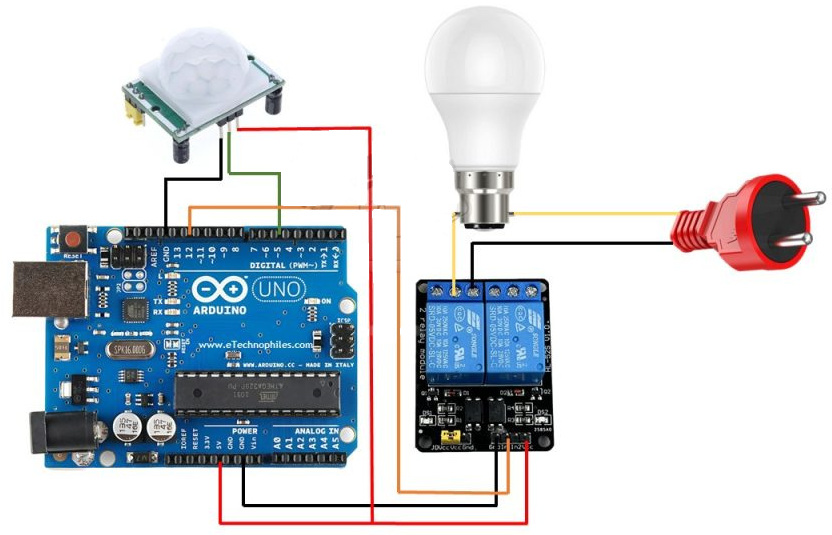
\includegraphics[width=0.6\textwidth]{imagem/Proj001}
	\caption{Esquemático para o Projeto 1}
\end{figure}

\begin{lstlisting}
// Definicao dos Pinos
#define PIR_PIN 5     // Digital para o Sensor PIR
#define RELAY_PIN 12  // Digital para o relay

// Tempo em millisegundos de espera para desligar o Relay
unsigned long motionTimeout = 3000;  
unsigned long lastMotionTime = 0;

// Inicializacao dos componentes
void setup() {
  pinMode(PIR_PIN, INPUT);
  pinMode(RELAY_PIN, OUTPUT);
  // Assegura que o relay esta desligado
  // (Lógica Reversa)
  digitalWrite(RELAY_PIN, HIGH);  
}

void loop() {
  // Ler o estado do PIR
  int pirState = digitalRead(PIR_PIN);
	
  if (pirState == HIGH) { // Movimento detectado
	// Liga o Relay (Logica Reversa)	
	digitalWrite(RELAY_PIN, LOW);
	// Atualiza a variavel de deteccao
	lastMotionTime = millis();     
	Serial.println("Motion detected: Relay ON");
  } else {
	// Sem movimento, verifica o tempo para apagar o relay
	if (millis() - lastMotionTime > motionTimeout) {
  	  // Desliga o relay (logica reversa)
	  digitalWrite(RELAY_PIN, HIGH);  
	}
  }
  // Espera 0,5 seg
  delay(500);
}
\end{lstlisting}

\subsection{Projeto 2 - Sistema de Rega Automática}

Este sensor com formato de garfo possui dois condutores que ao ser enterrado no solo consegue medir a umidade através da conexão entre os dois polos, um solo seco não conduzirá qualquer corrente elétrica entre os polos, diferente de um solo úmido, isso é obtido através de um comparador LM393.

\begin{figure}[H]
	\centering
	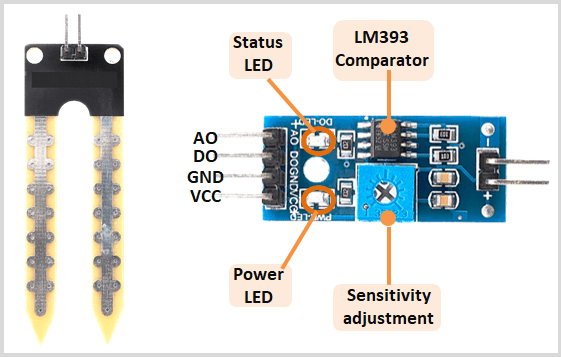
\includegraphics[width=0.6\textwidth]{imagem/soilsensor}
	\caption{Sensor para Umidade de Solo}
\end{figure}

Este projeto possui os seguintes materiais: \vspace{-1em}
\begin{itemize}
	\item Sensor para Umidade de Solo
	\item Bomba d'água com fonte de alimentação
	\item Mangueira de silicone para água
	\item Módulo Relay	
	\item Vasos que desejamos medir a umidade
\end{itemize}

\begin{figure}[H]
	\centering
	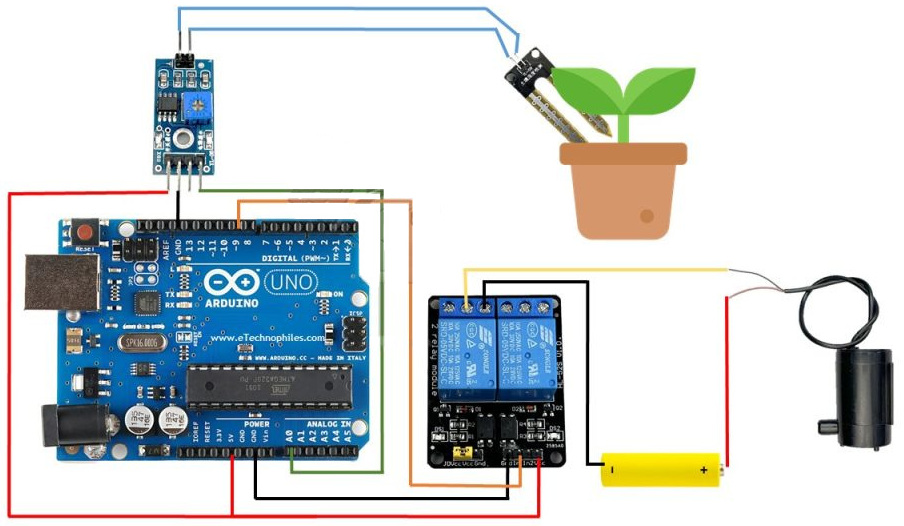
\includegraphics[width=0.6\textwidth]{imagem/Proj002}
	\caption{Esquemático para o Projeto 2}
\end{figure}

\begin{lstlisting}
// Definicao dos Pinos
const int SENSOR_SOIL = A0;  // Sensor Umidade de Solo
const int RELAY_PUMP = 9;    // Pino da Bomba

// Inicializacao dos componentes
void setup() {
  pinMode(RELAY_PUMP, OUTPUT);
  // Assegura que o relay esta desligado
  digitalWrite(RELAY_PUMP, LOW);  
}

void loop() {
  // Le o valor do sensor de solo
  int soilValue = analogRead(SENSOR_SOIL);
  // Ajuste o valor para a umidade desejada
  
  if (SENSOR_SOIL > 1000) { // Solo Seco
  	// Liga a bomba
	digitalWrite(RELAY_PUMP, HIGH);
  } else { // Solo umido
    // Desliga a bomba
	digitalWrite(RELAY_PUMP, LOW);  
  }
  // Espera para a proxima leitura
  delay(50000); // 5 mins
}
\end{lstlisting}

\subsection{Projeto 3 - Detector de Cor RGB (Vermelho, Verde e Azul)}

Este projeto possui os seguintes materiais: \vspace{-1em}
\begin{itemize}
	\item Módulo Sensor de Cor (TCS3200)
	\item LED RGB
\end{itemize}

\begin{figure}[H]
	\centering
	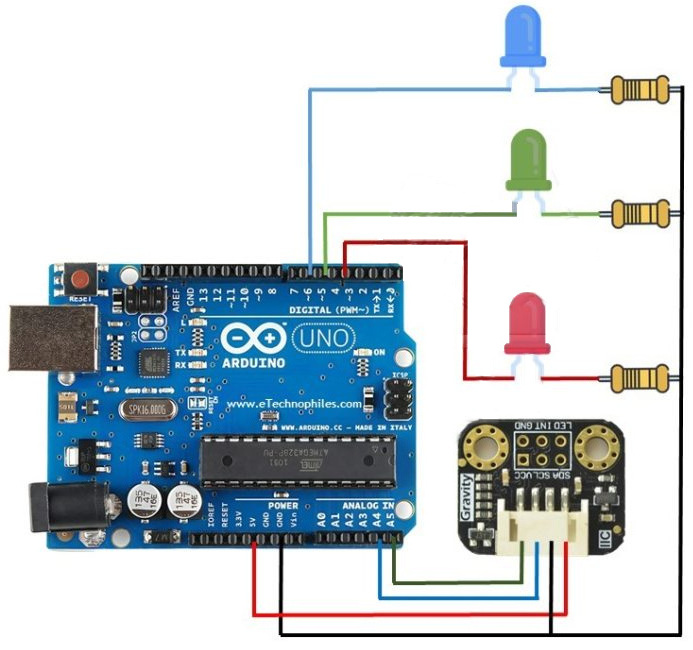
\includegraphics[width=0.6\textwidth]{imagem/Proj003}
	\caption{Esquemático para o Projeto 3}
\end{figure}

\begin{lstlisting}
// Biblioteca Necessaria	
#include <Wire.h>
#include "Adafruit_TCS34725.h"

// Definicao dos Pinos
#define RED_LED_PIN 3
#define GREEN_LED_PIN 5
#define BLUE_LED_PIN 6

// Criacao do objeto da biblioteca
Adafruit_TCS34725 tcs = 
  Adafruit_TCS34725(TCS34725_INTEGRATIONTIME_50MS, TCS34725_GAIN_4X);

void setup() {
  // Liga o sensor
  tcs.begin();
  
  // Inicializa os pinos do LED
  pinMode(RED_LED_PIN, OUTPUT);
  pinMode(GREEN_LED_PIN, OUTPUT);
  pinMode(BLUE_LED_PIN, OUTPUT);
	
  // Desliga todo o LED
  digitalWrite(RED_LED_PIN, LOW);
  digitalWrite(GREEN_LED_PIN, LOW);
  digitalWrite(BLUE_LED_PIN, LOW);
}

void loop() {
  // Variaveis para as cores	
  uint16_t r, g, b, c;
  // Obtem os dados
  tcs.getRawData(&r, &g, &b, &c);
	
  // Normaliza os valores RGB com as variáveis respectivas
  float red = r / (float)c * 255.0;
  float green = g / (float)c * 255.0;
  float blue = b / (float)c * 255.0;
	
  // Assegura os valores
  red = constrain(red, 0, 255);
  green = constrain(green, 0, 255);
  blue = constrain(blue, 0, 255);
	
  // Calcula a diferenca entre os valores
  float diffRG = abs(red - green);
  float diffRB = abs(red - blue);
  float diffGB = abs(green - blue);
	
  // Apaga o LED cuja diferenca menor que 50
  if (diffRG <= 50 && diffRB <= 50 && diffGB <= 50) {
	digitalWrite(RED_LED_PIN, LOW);
	digitalWrite(GREEN_LED_PIN, LOW);
	digitalWrite(BLUE_LED_PIN, LOW);
  } else {
	// Determine a cor dominant e liga para correspondencia do LED
	if (red > green && red > blue) {
	  digitalWrite(RED_LED_PIN, HIGH);
	  digitalWrite(GREEN_LED_PIN, LOW);
	  digitalWrite(BLUE_LED_PIN, LOW);
	} else if (green > red && green > blue) {
	  digitalWrite(RED_LED_PIN, LOW);
	  digitalWrite(GREEN_LED_PIN, HIGH);
	  digitalWrite(BLUE_LED_PIN, LOW);
	} else if (blue > red && blue > green) {
	  digitalWrite(RED_LED_PIN, LOW);
	  digitalWrite(GREEN_LED_PIN, LOW);
	  digitalWrite(BLUE_LED_PIN, HIGH);
	} else {
	  // Sem cor dominante apaga todos o LED
	  digitalWrite(RED_LED_PIN, LOW);
	  digitalWrite(GREEN_LED_PIN, LOW);
	  digitalWrite(BLUE_LED_PIN, LOW);
	}
  }
  // Espera 0,5 seg
  delay(500);
}
\end{lstlisting}

Variação para este projeto, sem usar o LED e apenas informações da Serial

\begin{lstlisting}
// Biblioteca Necessaria	
#include <Wire.h>
#include "Adafruit_TCS34725.h"

// Criar a tabela correlacional de Cores Gama
byte gammatable[256];
// Criar o objeto
Adafruit_TCS34725 tcs = Adafruit_TCS34725(TCS34725_INTEGRATIONTIME_50MS, TCS34725_GAIN_4X);

void setup() {
  // Liga a saida serial para mensagens
  Serial.begin(9600);
  // Verifica se o sensor foi ligado corretamente	
  if (!tcs.begin()) {
    Serial.println("TCS34725 não encontrado... Verifique as conexões");
	while (1);
  }
  // Tabela Correlacional de Cores Gama
  for (int i = 0; i < 256; i++) {
	float x = i / 255.0;
	x = pow(x, 2.5);
	x *= 255.0;
	gammatable[i] = commonAnode ? 255 - x : x;
  }
}

void loop() {
  // Variaveis para as cores	
  uint16_t r, g, b, c;
  // Obtem os dados
  tcs.getRawData(&r, &g, &b, &c);

  // Normaliza os valores RGB com as variáveis respectivas
  float red = r / (float)c * 255.0;
  float green = g / (float)c * 255.0;
  float blue = b / (float)c * 255.0;

  // Assegura os valores
  red = constrain(red, 0, 255);
  green = constrain(green, 0, 255);
  blue = constrain(blue, 0, 255);

  // Mostra os valores na saida da serial
  Serial.print("R:\t");
  Serial.print((int)red);
  Serial.print("\tG:\t");
  Serial.print((int)green);
  Serial.print("\tB:\t");
  Serial.print((int)blue);
  Serial.print("\tC:\t");
  Serial.println(c);

  // Espera 0,5 seg
  delay(500);
}	
\end{lstlisting}

\subsection{Projeto 4 - Sensor de Água}
Este sensor pode detectar a presença de água por medir a condutividade entre dois terminais metálicos (Metal Leads). Nesses sensores, os "leads" são geralmente as trilhas expostas na placa. Quando a água toca essas trilhas, cria um caminho elétrico entre elas, alterando a resistência que o sensor lê.

Este projeto possui os seguintes materiais: \vspace{-1em}
\begin{itemize}
	\item Módulo Sensor de Água
	\item Buzzer
	\item LED Vermelho
	\item Resistor de 220 $\Omega$
\end{itemize}

\begin{figure}[H]
	\centering
	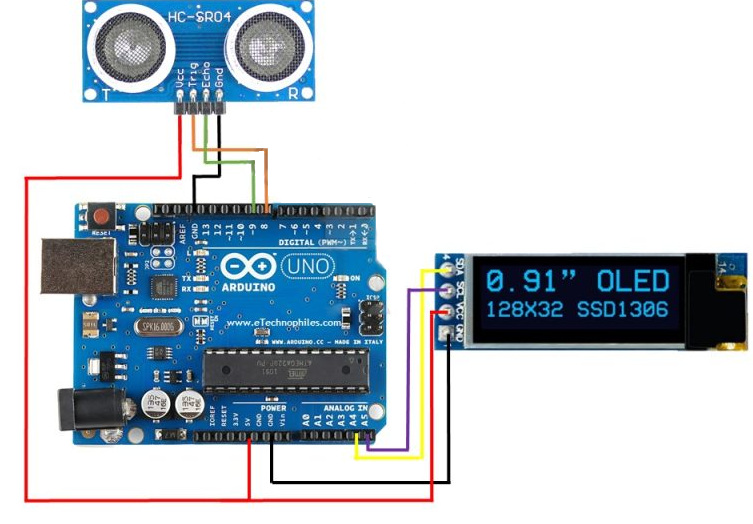
\includegraphics[width=0.4\textwidth]{imagem/Proj005}
	\caption{Esquemático para o Projeto 4}
\end{figure}

\begin{lstlisting}
// Definicao dos Pinos
#define WATER_SENSOR A0
#define LED 8
#define BUZZER 11

// Para ajustar o detector
const int threshold = 300;

void setup() {
  // Inicializa os pinos do LED e do Buzzer
  pinMode(LED, OUTPUT);
  pinMode(BUZZER, OUTPUT);
}

void loop() {
  // Le o valor do sensor
  int waterValue = analogRead(waterSensorPin);
  // Se existe agua (ajuste a variavel para melhor deteccao)
  if (waterValue > threshold) {
  	// Liga o LED
	digitalWrite(ledPin, HIGH);
  	// Liga o BUZZER
	digitalWrite(buzzerPin, HIGH);
  } else {
  	// Desliga o LED
    digitalWrite(ledPin, LOW);
  	// Desliga o Buzzer
	digitalWrite(buzzerPin, LOW);
  }
  // Espera 0,5 seg
  delay(500);
}
\end{lstlisting}

\subsection{Projeto 5 - Sensor Ultrassônico}
O sensor ultrassônico \textbf{HC-SR04} mede a distância enviando pulsos ultrassônicos e cronometrando quanto tempo eles levam para retornar. Neste projeto mediremos a distância de um objeto em relação a este sensor e exibiremos a distância em um display OLED de 0,91 polegadas. Possui os seguintes materiais: \vspace{-1em}
\begin{itemize}
	\item Módulo Ultrassônico HC-SR04
	\item Display OLED de 0.91 (128x32 px) polegadas
\end{itemize}

\begin{figure}[H]
	\centering
	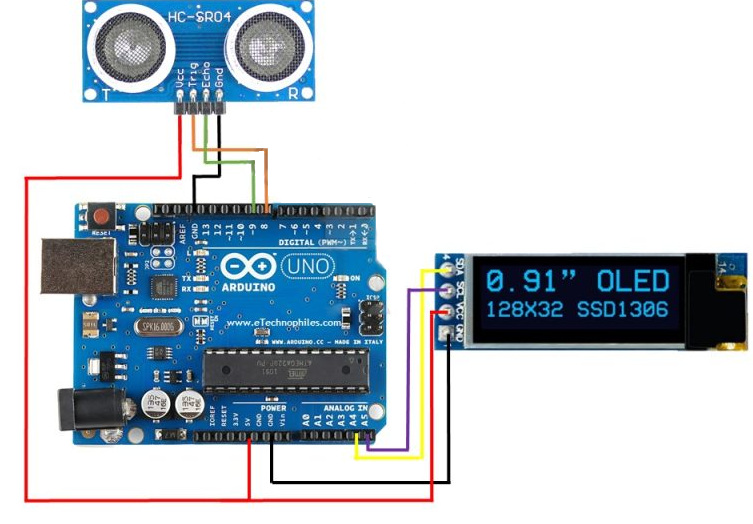
\includegraphics[width=0.6\textwidth]{imagem/Proj005}
	\caption{Esquemático para o Projeto 6}
\end{figure}

\begin{lstlisting}
// Biblioteca Necessaria	
#include <Wire.h>
#include <Adafruit_SSD1306.h>

// Pinos para o Display OLED
#define SCREEN_WIDTH 128
#define SCREEN_HEIGHT 32

// Pinos para o HC-SR04
#define TRIG_PIN 8
#define ECHO_PIN 9

Adafruit_SSD1306 display(SCREEN_WIDTH, SCREEN_HEIGHT, &Wire, -1);

void setup() {
  // Inicializa o Display OLED
  display.begin(SSD1306_SWITCHCAPVCC, 0x3C)
  display.clearDisplay();
  display.setTextSize(1);
  display.setTextColor(SSD1306_WHITE);
  display.setCursor(0, 0);
  display.println("HC-SR04 + OLED");
  display.setCursor(0, 16);
  display.println("Distance in cm");
  display.display();
  delay(2000);
  display.clearDisplay();
	
  // Initialize HC-SR04 pins
  pinMode(TRIG_PIN, OUTPUT);
  pinMode(ECHO_PIN, INPUT);
}

void loop() {
  long duration;
  float distance;
	
  // Envia um pulso de 10 segs
  digitalWrite(TRIG_PIN, LOW);
  delayMicroseconds(2);
  digitalWrite(TRIG_PIN, HIGH);
  delayMicroseconds(10);
  digitalWrite(TRIG_PIN, LOW);
	
  // Le o Eco e calcula a duracao
  duration = pulseIn(ECHO_PIN, HIGH);

  // Calcula a distancia em centimetros (velocidade do som = 34300 cm/s)
  distance = duration * 0.034 / 2;
	
  //Display distance on OLED
  display.clearDisplay();
  display.setCursor(0, 0);
  display.setTextSize(1);
  display.println("HC-SR04 Distancia");
  display.setTextSize(4);
  display.setCursor(0, 0);
  display.print(distance);
  display.print(" cm");
  display.display();
  
  // Espera 1 seg
  delay(1000);
}
\end{lstlisting}

\subsection{Projeto 6 - Sensor de Som}
Um módulo sensor de som geralmente inclui um microfone e um circuito amplificador, permitindo medir a intensidade das ondas sonoras. É perfeito para projetos que reagem a palmas, música ou ruído ambiente. Como neste projeto que os LEDs ligam e desligam conforme os níveis sonoros. Possui os seguintes materiais: \vspace{-1em}
\begin{itemize}
	\item Sensor de Som
	\item 3 LEDs de cores diferentes
	\item 3 Resistores de 220 $\Omega$
\end{itemize}

\begin{figure}[H]
	\centering
	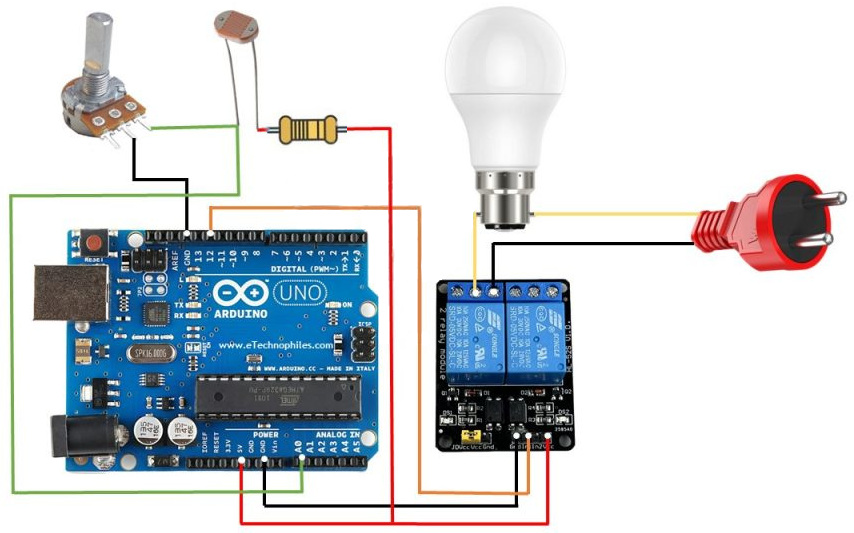
\includegraphics[width=0.6\textwidth]{imagem/Proj007}
	\caption{Esquemático para o Projeto 6}
\end{figure}

\begin{lstlisting}
// Pinos para o Display OLED
#define SOUND_SENSOR 2
#define LED_RED 3
#define LED_GREEN 5
#define LED_BLUE 6

void setup() {
  // Inicializa os pinos do LED e do Buzzer
  pinMode(LED_RED, OUTPUT);
  pinMode(LED_GREEN, OUTPUT);
  pinMode(LED_BLUE, OUTPUT);
}

void loop() {
  // Mede a altura do som
  int soundValue = digitalRead(SOUND_SENSOR);
  // Desliga todos os LEDs
  digitalWrite(LED_RED, LOW);
  digitalWrite(LED_GREEN, LOW);
  digitalWrite(LED_BLUE, LOW);
  // Liga os LEDs conforme o valor (ajustar)
  if (soundValue > 100) {
  	digitalWrite(LED_RED, HIGH);
  }
  if (soundValue > 200) {
	digitalWrite(LED_GREEN, HIGH);
  }
  if (soundValue > 300) {
	digitalWrite(LED_BLUE, HIGH);
  }
  delay(100);
}	
\end{lstlisting}

\subsection{Projeto 7 - LDR (Light Dependent Resistor)}
Neste projeto usamos um LDR para detectar a escuridão e ligar automaticamente uma lâmpada conectada a um módulo relé. Este projeto é comumente utilizado em sistemas de iluminação para economia de energia. Possui os seguintes materiais: \vspace{-1em}
\begin{itemize}
	\item LDR
	\item Resistor de 10 K$\Omega$ (para agir como divisor de voltagem do LDR)
	\item Lâmpada com seu conector
	\item Módulo Relay
\end{itemize}

\begin{figure}[H]
	\centering
	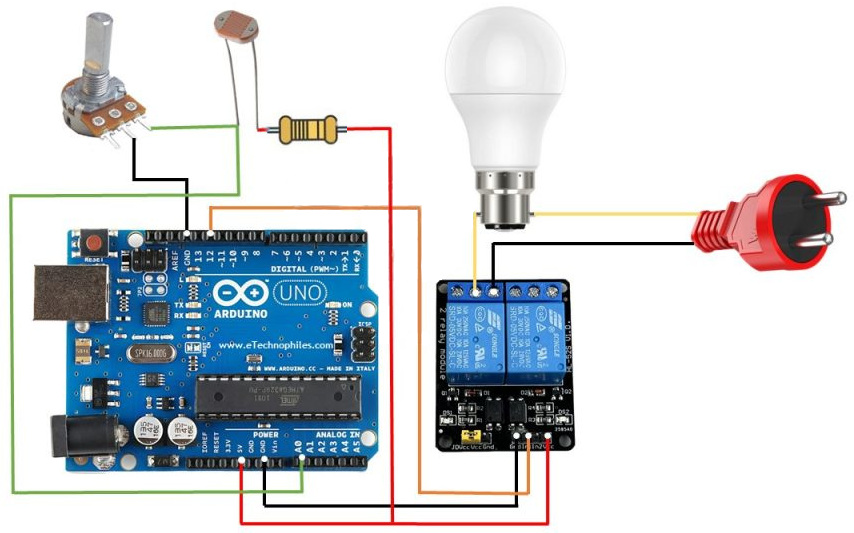
\includegraphics[width=0.6\textwidth]{imagem/Proj007}
	\caption{Esquemático para o Projeto 8}
\end{figure}

\begin{lstlisting}
// Pinos para o LDR e o RELAY
#define LDR_PIN A0
#define RELAY_PIN 12

// Define o valor que a lampada deve acender
int threshold = 450;

void setup() {
  // Configurar o RELAY
  pinMode(RELAY_PIN, OUTPUT);
  digitalWrite(RELAY_PIN, HIGH);
}

void loop() {
  // Ler o valor do LDR
  int ldrValue = analogRead(LDR_PIN);
  // Controla o relay com base no valor
  if (ldrValue < threshold) {
 	// Se nivel de luz e baixo liga o Relay
	digitalWrite(RELAY_PIN, LOW);
  } else {
 	// Se nivel de luz e alto desliga o Relay
	digitalWrite(RELAY_PIN, HIGH);
  }
  // Espera 0,5 seg
  delay(500);
}	
\end{lstlisting}

\section{Sensores IR}

\subsection{Projeto 8 - Sensor IR (Receptor Infravermelho)}
Um controle remoto possui um LED Infravermelho que produz um pulso de luz infravermelha que envia os sinais para um IR que decodifica esses. O IR contém um fotodiodo que amplifica e converte os sinais de luz em pulsos elétricos.

\begin{figure}[H]
	\centering
	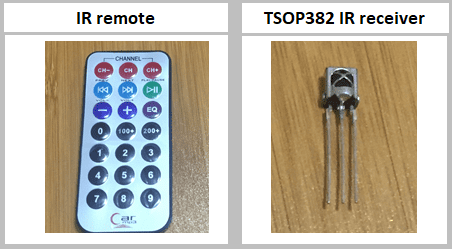
\includegraphics[width=0.6\textwidth]{imagem/controle}
	\caption{Controle Remoto e Receptor Infravermelho}
\end{figure}

Este projeto possui os seguintes materiais: \vspace{-1em}
\begin{itemize}
	\item Módulo TSOP382 IR Receiver
	\item Lâmpada com seu conector
	\item Módulo Relay com 2 canais
	\item Motor DC
	\item Fonte de alimentação para o Motor
	\item Controle remoto para enviar informações para o IR
\end{itemize}

\begin{figure}[H]
	\centering
	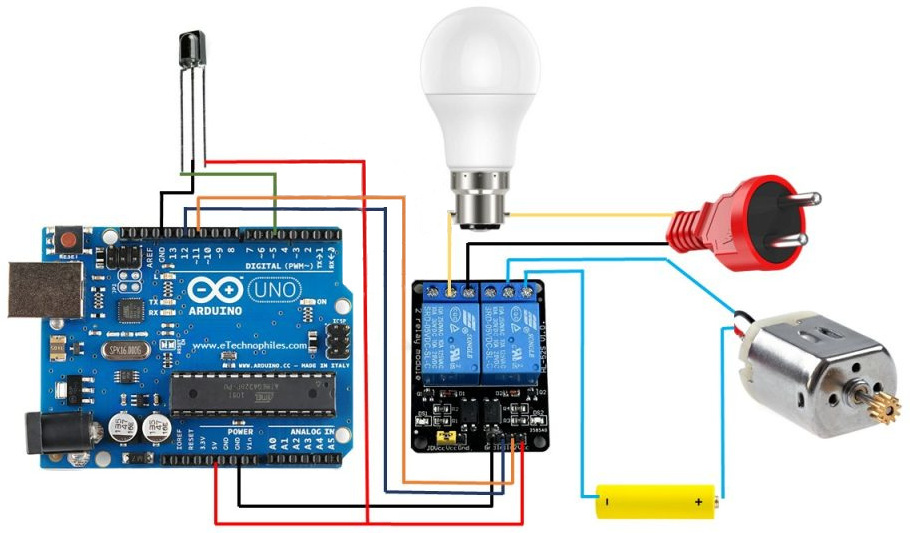
\includegraphics[width=0.6\textwidth]{imagem/Proj_IR01}
	\caption{Esquemático para o Projeto 8}
\end{figure}

Primeiro, todo IR exige um controle para enviar a informação, e cada controle funciona com um padrão Hexadecimal de valores, assim precisamos primeiro conhecer esse padrão para ligar e desligar os elementos, esse simples programa irá mostrar esses valores:

\begin{lstlisting}
	#include <IRremote.h>
	
	// Definicao dos Pinos
	#define IR_RECEIVE_PIN 5
	
	// Inicializacao do IR
	IRrecv irrecv(IR_RECEIVE_PIN);
	decode_results results;
	
	void setup() {
		// Inicializa a Serial
		Serial.begin(115200);
		
		// Inicializa o IR
		Serial.println("Habilita IR");
		irrecv.enableIRIn();
		
		Serial.println("IR pronto para receber os sinais");
	}
	
	void loop() {
		if (irrecv.decode(&results)) {
			Serial.print("Received code: ");
			Serial.println(results.value, HEX);
		}
		// Espera 0,1 seg
		delay(100);
	}	
\end{lstlisting}

Selecione 2 botões a sua escolha no controle remoto e anote os valores que aparecem no monitor da saída serial.

\begin{lstlisting}
	#include <IRremote.h>
	
	// Definicao dos Pinos
	#define IR_RECEIVE_PIN 5
	#define RELAY1_PIN 11
	#define RELAY2_PIN 12
	
	// Inicializacao do IR
	IRrecv irrecv(IR_RECEIVE_PIN);
	decode_results results;
	
	// Definir os códigos para o IR (ajustar com o controle)
	#define BUTTON_1 0xFF30CF  // PRIMEIRO CÓDIGO HEX para o botao 1
	#define BUTTON_2 0xFF18E7  // SEGUNDO CÓDIGO HEX para o botao 2
	
	// Estado do Relay
	bool relay1State = false;
	bool relay2State = false;
	
	void setup() {
		// Inicializa os pinos do Relay
		pinMode(RELAY1_PIN, OUTPUT);
		pinMode(RELAY2_PIN, OUTPUT);
		
		// Assegura que o Relay esta desligado
		// (Logica reversa)
		digitalWrite(RELAY1_PIN, HIGH);
		digitalWrite(RELAY2_PIN, HIGH);
		
		// Inicializa o IR
		irrecv.enableIRIn();
	}
	
	void loop() {
		if (irrecv.decode(&results)) {
			// Verifica o recebimento
			if (results.value == BUTTON_1) {
				digitalWrite(RELAY1_PIN, relay1State);
				relay1State = !relay1State;  // Muda o estado do Canal 1 do Relay
			} else if (results.value == BUTTON_2) {
				digitalWrite(RELAY2_PIN, relay2State);
				relay2State = !relay2State;  // Muda o estado do Canal 2 do Relay
			}
			irrecv.resume(); // Recebe o proximo valor
		}
		// Espera 0,1 seg
		delay(100);
	}	
\end{lstlisting}

\subsection{Projeto 9 - Sensor de Obstáculo IR}
Os sensores de desvio de obstáculos IR (infravermelho) usam luz infravermelha para detectar obstáculos sem contato físico. São elementos comuns na robótica, especialmente para navegação autônoma. Neste projeto criamos um alarme contra intrusos, posicione o sensor próximo a portas ou janelas. Quando um intruso se aproxima, o sensor detecta um objeto dentro de um determinado alcance e dispara um alarme.

Este projeto possui os seguintes materiais: \vspace{-1em}
\begin{itemize}
	\item Módulo Sensor IR de Obstáculos
	\item Buzzer
	\item Resistor de 220 $\Omega$
\end{itemize}

\begin{figure}[H]
	\centering
	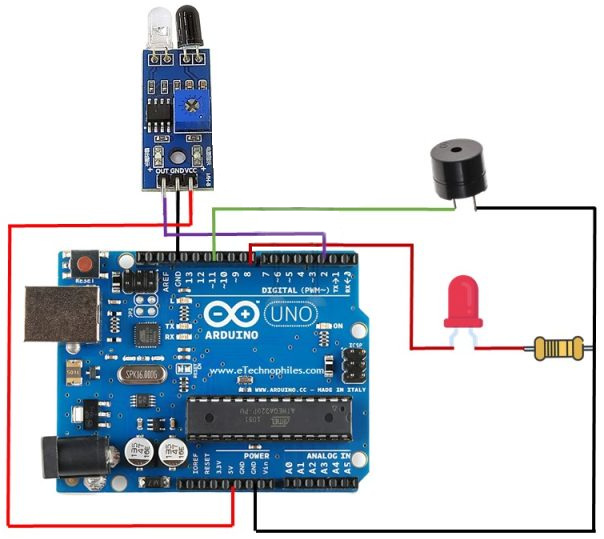
\includegraphics[width=0.5\textwidth]{imagem/Proj_IR02}
	\caption{Esquemático para o Projeto 9}
\end{figure}

\begin{lstlisting}
// Definicao dos Pinos
#define IR_SENSOR 2 // Sensor IR
#define LED 8       // LED
#define BUZZER 11   // Buzzer

void setup() {
  // Inicializar as entradas e saidas
  pinMode(IR_SENSOR, INPUT); // Sensor IR de entrada
  pinMode(LED, OUTPUT);      // LED de saida
  pinMode(BUZZER, OUTPUT);   // Buzzer de saida
}

void loop() {
  // Le o valor do sensor
  int irValue = digitalRead(IR_SENSOR);
  // Objeto detectado	
  if (irValue == LOW) {
 	digitalWrite(LED, HIGH);    // Liga o LED
	digitalWrite(BUZZER, HIGH); // Liga o buzzer
  } else {
	digitalWrite(LED, LOW);     // Desliga o LED
	digitalWrite(BUZZER, LOW);  // Desliga o buzzer
  }
  delay(500); // Espera de 0,5 seg
}	
\end{lstlisting}

\subsection{Projeto 10 - Estacionamento Inteligente}
Agora que conhecemos esse sensor, vamos construir um projeto mais "acadêmico" (ideal para qualquer "Feira de Ciências"). Um sistema inteligente de estacionamento ajuda a resolver um problema comum: encontrar vagas em áreas com grande fluxo de veículos, como áreas residenciais, prédios comerciais, escolas e outras instalações.

Este projeto possui os seguintes materiais: \vspace{-1em}
\begin{itemize}
	\item 8 módulos Sensor IR de Obstáculos
	\item 2 servos motor
	\item Cartolina para criar o estacionamento
	\item Carros de brinquedo
\end{itemize}

\begin{figure}[H]
	\centering
	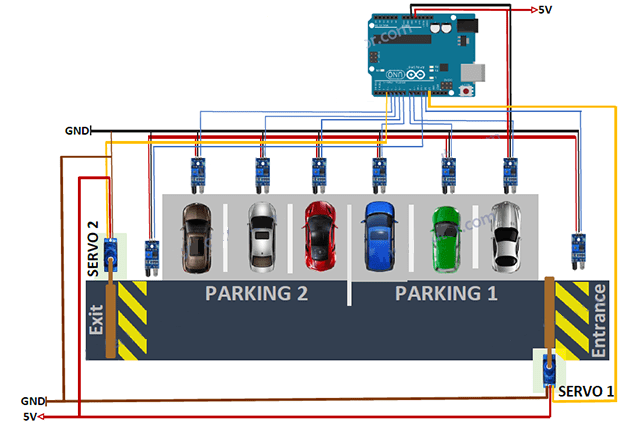
\includegraphics[width=0.8\textwidth]{imagem/Proj_IR03}
	\caption{Esquemático para o Estacionamento Inteligente}
\end{figure}

\begin{lstlisting}
#include <Servo.h>

// Posicoes das vagas
#define SLOT1 4
#define SLOT2 5
#define SLOT3 6
#define SLOT4 7
#define SLOT5 8
#define SLOT6 9
// Portoes
#define ENTRANCE 11
#define EXIT 12

// Objetos para o controle dos Servos
Servo myservo1;  
Servo myservo2;

int pos1 = 90;  // Giro do Portao de entrada
int pos2 = 90;  // Giro do Portao de saida

// Dados Completos, consiste nos valores dos sensores
String cdata =""; 

void setup() {
  // Para as vagas
  pinMode(SLOT1, INPUT);
  pinMode(SLOT2, INPUT);
  pinMode(SLOT3, INPUT);
  pinMode(SLOT4, INPUT);
  pinMode(SLOT5, INPUT);
  pinMode(SLOT6, INPUT);

  // Para os portoes  
  pinMode(ENTRANCE, INPUT);
  pinMode(EXIT, INPUT);
  
  // Para os Servos
  myservo1.attach(13);  
  myservo2.attach(3);
}

void loop() {
  verify_gates();
  delay(6000);
}

// Para os portoes
void verify_gates() {
  // Sensor do portao de saida	
  // Carro parado no portao de saida (LOW)
  if (digitalRead(EXIT) == LOW) {
  	// Faz o servo ir de 90 a 180 graus
  	// Observar no esquematico a posicao desse servo
    for (pos2 = 90; pos2 <= 180 ; pos2 += 1) {
      myservo2.write(pos2);
      delay(15);
    }
    delay(1000);
  	// Faz o servo voltar a posicao atual de 90 graus
    for (pos2 = 180; pos2 >= 90; pos2 -= 1) {
      myservo2.write(pos2);
      delay(15);
    }
  }
  
  // Sensor do portao de entrada
  // Carro parado no portao de entrada (LOW)
  // e existe alguma vaga disponivel (sensor em HIGH)
  if ((digitalRead(ENTRANCE) == LOW) && (
      (digitalRead(SLOT1) == HIGH) || 
      (digitalRead(SLOT2) == HIGH) || 
      (digitalRead(SLOT3) == HIGH) || 
      (digitalRead(SLOT4) == HIGH) || 
      (digitalRead(SLOT5) == HIGH) || 
      (digitalRead(SLOT6) == HIGH) )) {
  	// Faz o servo ir de 0 a 90 graus
  	// Observar no esquematico a posicao desse servo
    for (pos1 = 0; pos1 <= 90 ; pos1 += 1) {
      myservo1.write(pos1);
      delay(15);
    }
    delay(1000);
  	// Faz o servo voltar a posicao atual de 0 graus
    for (pos1 = 90; pos1 >= 0; pos1 -= 1) {
      myservo1.write(pos1);
      delay(15);
    }
  }
}
\end{lstlisting}

\subsection{Projeto 11 - Detector de Velocidade}
Como as barreiras eletrônicas (populares "pardais") medem a velocidade de veículos em movimento ou como a velocidade de uma corrida de um atleta é registrada? Normalmente, esses sensores de velocidade funcionam com tecnologia de radar ou laser, refletindo ondas de rádio ou luz infravermelha nos objetos e calculando a velocidade com base no tempo que a onda ou a luz leva para retornar.

Ao posicionar dois sensores IR a uma distância fixa um do outro, podemos medir o tempo que um objeto leva para se deslocar entre eles. Com o tempo registrado e a distância conhecida entre os sensores, é possível calcular com precisão a velocidade do objeto por meio de uma fórmula.

Este projeto possui os seguintes materiais: \vspace{-1em}
\begin{itemize}
	\item 2 módulos Sensor IR de Obstáculos
	\item Display LCD I2C - 16x2
\end{itemize}

\begin{figure}[H]
	\centering
	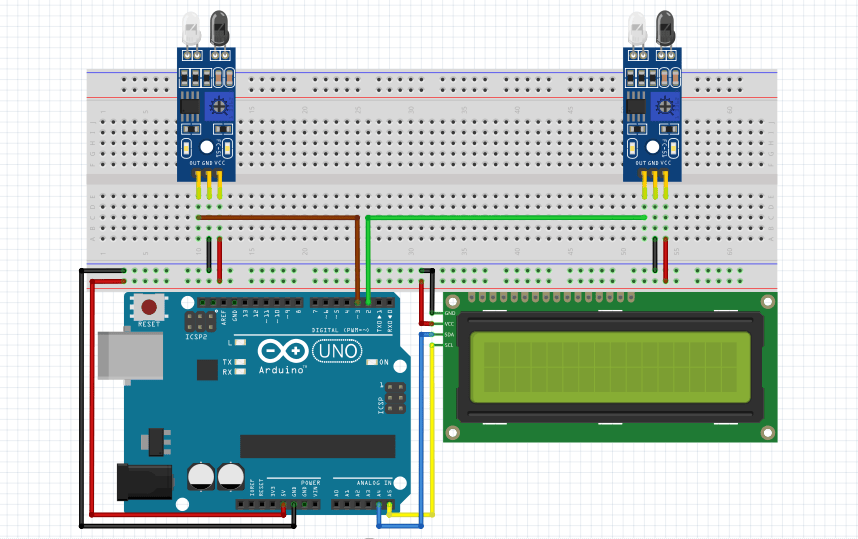
\includegraphics[width=0.7\textwidth]{imagem/Proj_IR04}
	\caption{Esquemático para o Projeto 10}
\end{figure}

No esquemático devemos observar que os dois sensores devem estar a uma distância correta, neste caso usaremos 10 cm, utilizamos uma régua para acertar corretamente essa medida

\begin{figure}[H]
	\centering
	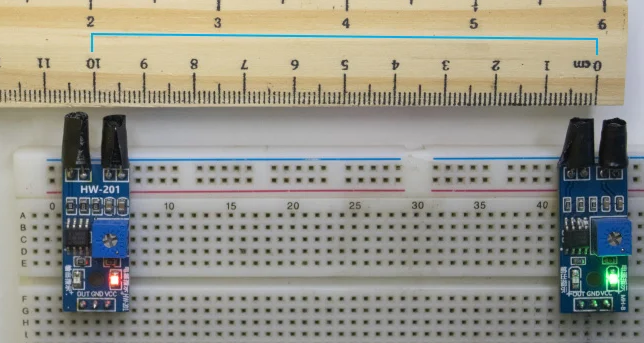
\includegraphics[width=0.6\textwidth]{imagem/distancia}
	\caption{Distância entre os sensores}
\end{figure}

Como conhecemos a distância entre os dois sensores IR. Precisamos apenas saber o tempo que o objeto leva para passar de um sensor ao outro, e podemos facilmente determinar a velocidade do objeto em movimento utilizando a “fórmula da velocidade”.

Velocidade = Distância entre dois sensores IR / Tempo gasto pelo objeto para percorrer a distância entre os dois sensores

Por exemplo, se a distância (d) entre os dois sensores IR for de 1 metro e o objeto levar um tempo (t) de 0,4 segundos para se deslocar entre eles, então a velocidade será: $V = \nicefrac{d}{t} = \nicefrac{1}{0,4} = 2,5 m/s$

\begin{lstlisting}
\\ Bibliotecas necessarias
#include <Wire.h>
#include <LiquidCrystal_I2C.h>

// Inicializacao do LCD por padrao no endereco (0x27 ou 0x3F)
LiquidCrystal_I2C lcd(0x27, 16, 2);	

// Posicao dos sensores IR
#define SENSOR_1_PIN 2
#define SENSOR_2_PIN 3

// Variaveis locais
volatile unsigned long timeSensor1 = 0;
volatile unsigned long timeSensor2 = 0;
volatile bool sensor1Triggered = false;
volatile bool sensor2Triggered = false;
// Distancia entre os sensores, em Mt
const float distanceBetweenSensors = 0.1; 
// Velocidade em metros por segundo (m/s)
float speed = 0; 

void setup() {
  // Initialize the LCD
  lcd.init();
  lcd.backlight();
  // Mostrar o titulo
  lcd.setCursor(0, 0);
  lcd.print("Radar de Velocidade");
  delay(2000);
  lcd.clear();
  pinMode(SENSOR_1_PIN, INPUT);
  pinMode(SENSOR_2_PIN, INPUT);
  // Acessar a acao para os sensores 1 (INT0) e 2 (INT1)
  attachInterrupt(digitalPinToInterrupt(SENSOR_1_PIN), sensor1ISR, RISING);
  attachInterrupt(digitalPinToInterrupt(SENSOR_2_PIN), sensor2ISR, RISING);
}

void loop() {
  if (sensor1Triggered && sensor2Triggered) {
    sensor1Triggered = false;
	sensor2Triggered = false;
	// Tempo em microsegundos
	unsigned long timeDifference = abs(timeSensor2 - timeSensor1);
	lcd.clear();
	if (timeDifference > 0) {
	  // Converter para segundos
	  speed = distanceBetweenSensors / (timeDifference / 1000000.0);
      // Posicionar na Linha 1
	  lcd.setCursor(0, 0);
	  lcd.print("Velocidade:");
      // Posicionar na Linha 2
	  lcd.setCursor(0, 1);
	  // Mostrar com 2 casas decimais
	  lcd.print(speed, 2);
	  lcd.print(" m/s");
	} else {
	  lcd.setCursor(0, 0);
	  lcd.print("Leitura Incorreta!");
	}
  }
}

void sensor1ISR() {
  // Assegura que o primeiro ponto nao foi gravado
  if (!sensor1Triggered) {
  	// Registra o tempo do 1o. Sensor
    timeSensor1 = micros();
	sensor1Triggered = true;
  }
}
void sensor2ISR() {
  // Assegura que o segundo ponto nao foi gravado
  if (!sensor2Triggered) {
  	// Registra o tempo do 2o. Sensor
	timeSensor2 = micros();
	sensor2Triggered = true;
  }
}	
\end{lstlisting}

\section{Micro SD Card (Secure Digital)}
Cartões de Segurança Digital são usados em uma variedade de aplicações. O módulo SD Card possui somente um único chip, um regulador de dropout ultrabaixo integrado que converte tensões de 3,3V a 6V em 3,3V, já que é a tensão padrão de operação desse módulo.

\subsection{Projeto 12 - Módulo Micro SD Card (Secure Digital)}
Diferentemente do Módulo Micro SD Card, o módulo acima não possui conversão de tensão para todos os sinais lógicos, portanto, na montagem do projeto, será necessário aplicar uma divisão de tensão nas entradas para convertermos a tensão de 5 V para 3,3 V. Também possui uma entrada para um cartão SD formatado em FAT32.

Este projeto possui os seguintes materiais: \vspace{-1em}
\begin{itemize}
  \item Módulo Micro SD Card
  \item Cartão de Memória MicroSD
  \item Resistor de 330 $\Omega$
  \item Resistor de 680 $\Omega$
\end{itemize}

\begin{figure}[H]
  \centering
  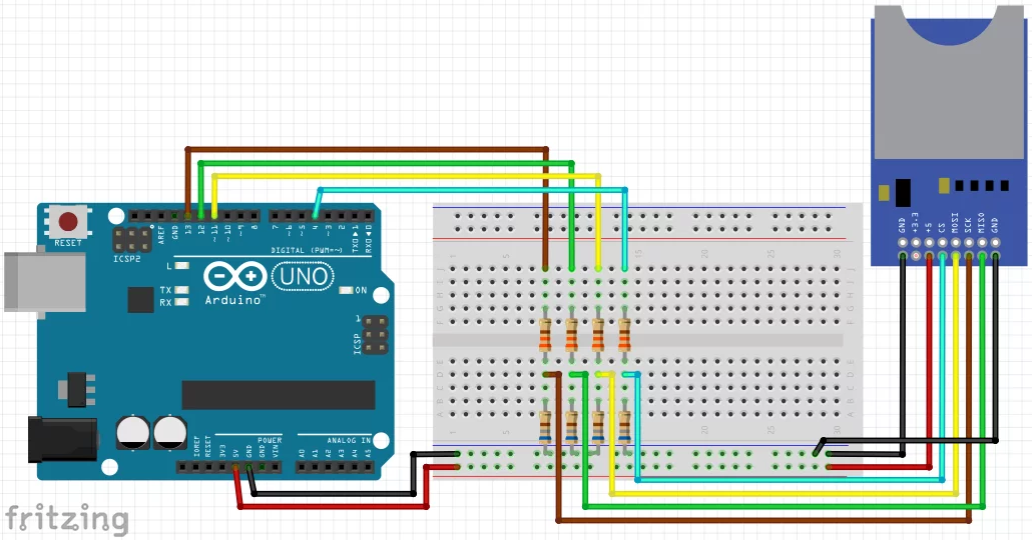
\includegraphics[width=0.5\textwidth]{imagem/Proj_card01}
  \caption{Esquemático para o Projeto 12}
\end{figure}

\begin{lstlisting}
/*
cartão SD conectado ao SPI da seguinte maneira:
 MOSI - pino 11
 MISO - pino 12
 CLK  - pino 13
 SDCS - pino 4
*/
#include <SPI.h>
#include <SD.h>

File myFile;

void setup() {
  Serial.begin(9600);
  while (!Serial) {
    ; // Espera a porta serial conectar
  }
  Serial.print("Inicializando cartão SD...");
  if (!SD.begin(4)) {
    Serial.println("Falha na inicialização!");
  while (1);
  }
  Serial.println("Inicialização feita.");
  
  // Abre o arquivo. Perceba que apenas um arquivo pode ser aberto nesse momento,
  // portanto você terá que fechar este antes de abrir outro
  myFile = SD.open("test.txt", FILE_WRITE);
  
  // Se este arquivo abriu corretamente, escreva nele:
  if (myFile) {
    Serial.print("Escrevendo para test.txt...");
  myFile.println("testando 1, 2, 3.");
  // fecha o arquivo:
  myFile.close();
  Serial.println("feito.");
  } else {
    // Se este arquivo não abriu, imprima um erro:
  Serial.println("Erro ao abrir test.txt");
  }
  // Abre novamente o arquivo para leitura:
  myFile = SD.open("test.txt");
  if (myFile) {
    Serial.println("test.txt:");
  // Lê do arquivo até não ter mais nada nele:
  while (myFile.available()) {
      Serial.write(myFile.read());
  }
  // fecha o arquivo:
  myFile.close();
  } else {
  // Se este arquivo não abriu, imprima um erro:
  Serial.println("Erro ao abrir test.txt");
  }
}

void loop() {
  // Use este ponto para ser a base de coleta de dados para 
  // o cartão SD Card.
}  
\end{lstlisting}

\subsection{Projeto 13 - Micro SD Card com Sensor Ultrassônico}
O cartão micro SD com Arduino permite o desenvolvimento de dataloggers. Dispositivos que armazenam dados coletados de sensores e outros informações para análise e construção de gráficos.

Este projeto possui os seguintes materiais: \vspace{-1em}
\begin{itemize}
  \item Módulo Sensor de Distância Ultrassônico HC-SR04
  \item Módulo Micro SD Card
  \item Cartão de Memória MicroSD
  \item 3 Resistores de 3 K$\Omega$
  \item 3 Resistores de 2 K$\Omega$
\end{itemize}

\begin{figure}[H]
  \centering
  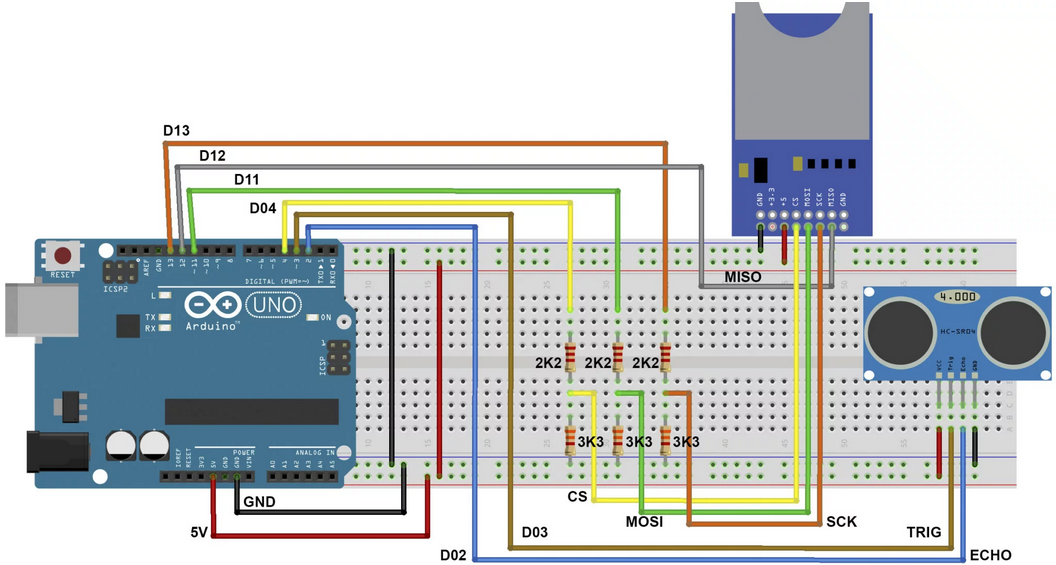
\includegraphics[width=0.7\textwidth]{imagem/Proj_card02}
  \caption{Esquemático para o Projeto 13}
\end{figure}

\begin{lstlisting}
#include <SPI.h>
#include <SD.h>
#include <stdlib.h>

// Definicao dos Pinos
#define CS 4 // Pino usado para o cartao
#define TRIG_PIN 3 // Pino usado para disparar os pulsos do sensor
#define ECHO_PIN 2 // pino usado para ler a saida do sensor

// Variaveis para cartao SD
char dataString[7];
File myFile;

void setup() {
  // configura pino de Trigger como saída e inicializa com nivel baixo
  pinMode(TRIG_PIN,OUTPUT);
  digitalWrite(TRIG_PIN,LOW); 
  pinMode(ECHO_PIN,INPUT);// configura pino ECHO como entrada
  pinMode(CS, OUTPUT);
  Serial.begin(9600);
  delay(100);
 
  Serial.print("Inicializando cartao SD...");
  if (!SD.begin(CS)) {
    Serial.println("Falha na Inicializacao!");
    return;
  }
  Serial.println("Inicializacao terminada");
}

void loop() {
  // Envia pulso para o disparar o sensor e retornar a distancia
  float val = pulse();
  // Adiciona a leitura na string de gravacao
  dtostrf(val,5,2,dataString);  
  if (meuArquivo = SD.open("log.txt",FILE_WRITE)) {
    Serial.print("Gravou: ");
  Serial.println(val);
  // Escreve no cartao SD por meio do objeto meuArquivo 
  myFile.println(dataString);
  myFile.close();
  } else {
  // Se o arquivo nao abrir, mostra msg de erro
  Serial.println("Erro ao abrir log.txt");
  }
  delay(2000);
}

// Funcao para enviar o pulso de trigger
float pulse() {
  long duration;
  float distance;

  // Envia um pulso de 10 segs
  digitalWrite(TRIG_PIN, LOW);
  delayMicroseconds(2);
  digitalWrite(TRIG_PIN, HIGH);
  delayMicroseconds(10);
  digitalWrite(TRIG_PIN, LOW);

  // Le o Eco e calcula a duracao
  duration = pulseIn(ECHO_PIN, HIGH);

  // Calcula a distancia em centimetros (velocidade do som = 34300 cm/s)
  distance = duration * 0.034 / 2;
  return distance;
}
\end{lstlisting}


\subsection{Projeto 14 - Micro SD Card com Calc (Libre Office)}
\textit{Data Logging} é uma técnica de dados que envolve coletar, analisar e interpretar os dados. Neste projeto vamos trabalhar com temperatura e umidade, levando nossos dados até o Calc (plataforma gratuita similar ao Excel).

Este projeto possui os seguintes materiais: \vspace{-1em}
\begin{itemize}
  \item Módulo DS3231 RTC
  \item Módulo Micro SD Card
  \item Cartão de Memória MicroSD
  \item Sensor de temperatura LM35
  \item LDR (\textit{Light Dependent Resistor})
  \item Resistor de 220 $\Omega$
\end{itemize}

\begin{figure}[H]
  \centering
  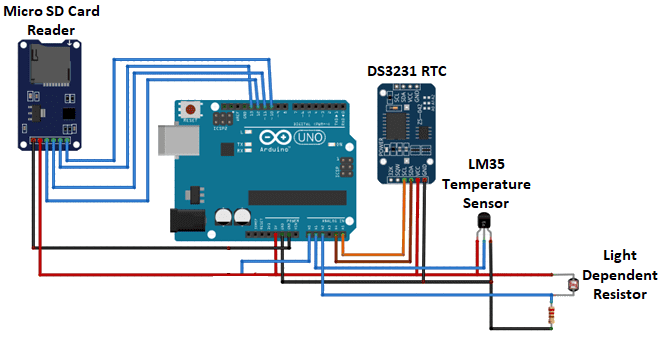
\includegraphics[width=0.7\textwidth]{imagem/Proj_card03}
  \caption{Esquemático para o Projeto 14}
\end{figure}

\begin{itemize}
  \item Módulo DS3231 RTC ligações no Arduino: GND -> GND; VCC -> VCC (5V); SDA -> A4; SCK -> A5
  \item Módulo Micro SD Card ligações no Arduino: GND -> GND; VCC -> VCC (5V); SCK -> Pino 13; MISO -> Pino 12; MOSI -> Pino 11; CS -> Pino 10
\end{itemize}

\begin{lstlisting}
#include <DS3231.h> 
#include <SPI.h> 
#include <SD.h> 

// Definicao dos Pinos
#define TMP A2
#define LDR A1

File dataFile; 

float temperature;
int light_percentage;

const int chipSelect = 10; //SD card CS pin connected to pin 10 of Arduino

// Inicializa o DS3231
DS3231 rtc(SDA, SCL);

void setup() {
  rtc.begin();
  Serial.begin(9600);
  
  // Iniciar a SD card
  Serial.print("Inicialização da SD card...");
  if (!SD.begin(chipSelect)) {
    Serial.println("inicialização falhou!");
    return;
  }
  Serial.println("Inicialização concluída.");
  
  // Abrir o arquivo
  dataFile = SD.open("LOGDATA.txt", FILE_WRITE);
  
  // Abrir e Escrever no arquivo:
  if (dataFile) {
    Serial.println("Arquivo aberto OK");
    // Adicionar o cabecalho aos dados
    dataFile.println("Data,Hora,Temperatura,Intensidade");
  }
  dataFile.close();

  // Mostra na saida da Serial  
  Serial.println("CLEARDATA"); // Limpa os dados
  Serial.println("LABEL,Data,Hora,Temperatura,Intensidade"); 
  // A palavra LABEL, indica a primeira linha
  Serial.println("RESETTIMER");
}

void loop() {
  int temp_sensor_val = analogRead(TMP);
  int ldr_sensor_val = analogRead(LDR);

  // Converte os valores de intensidade para a faixa de 0 a 100  
  int light_percentage = map(ldr_sensor_val, 0, 1023, 0, 100);
  
  // Calcula a temperatura em Graus Celcius
  float millivolts = (temp_sensor_val / 1024.0) * 5000;
  float temperature = millivolts / 10;
  
  dataFile = SD.open("LOGDATA.txt", FILE_WRITE);
  
  // Se o arquivo estah disponivel, gravar
  if (dataFile) {
    dataFile.print(rtc.getDateStr()); // Armazena a Data
    dataFile.print(","); // Move para a proxima coluna ","
    dataFile.print(rtc.getTimeStr()); // Armazena a hora
    dataFile.print(",");
    dataFile.print(temperature); // Armazena a temperatura
    dataFile.print(",");
    dataFile.print(light_percentage); // Armazena a Intensidade de Luz
    dataFile.println(); // Finaliza e move para a próxima linha
    dataFile.close(); //Close the file
    // Informa na serial
    Serial.println("Linha adicionada");
  } else
    Serial.println("OOPS!! SD card falhou para escrever");
  
  delay(5000); // Espera 5 segundos
}
\end{lstlisting}

Para analisar esses dados, precisamos abri-los no \textbf{Calc} como um arquivo CSV (\textit{Comma Separated Value} - Valores Separados por Vírgula). Para isso, sigamos seguintes passos abaixo:
\begin{enumerate}
  \item Abrir o \textbf{Calc} e clique em Arquivo > Abrir. 
  \item Selecionar o arquivo “LOGDATA.txt” a partir do cartão SD. Isso abrirá o Assistente de Importação de Texto.
  \item No assistente, escolher "Separado por" e marcar a opção Vírgula como delimitador. 
  \item Clicar em Avançar (se houver) e depois em OK ou Concluir.
  \item Os valores serão então abertos em uma planilha do \textbf{Calc}, com os dados registrados organizados em colunas.
\end{enumerate}

A forma como os valores são exibidos no \textbf{Calc} corresponde à maneira como foram gravados no \textbf{cartão SD}. No arquivo de texto, cada vírgula indica a passagem para a próxima coluna. Após importar os dados para a planilha do \textbf{Calc}, podemos realizar análises com a utilização dos diversos recursos disponíveis no \textbf{Calc}.

\section{Conclusão}
Aprender Arduino por meio de projetos práticos coloca o estudante em contato direto com problemas reais, estimulando a experimentação, a curiosidade e o raciocínio lógico. Em vez de apenas memorizar conceitos teóricos, o aluno constrói circuitos, programa sensores e observa o funcionamento dos sistemas em tempo real. Essa abordagem “mão na massa” (\textit{hands on}) facilita a compreensão de conteúdos como eletrônica básica, programação e lógica de controle, tornando o aprendizado mais concreto e significativo.

Esta abordagem prática e orientada por exemplos facilita o aprendizado e a inovação, permite a transição rápida da teoria para a construção de projetos eletrônicos reais e complexos, satisfaz tanto a curiosidade quanto a necessidade de soluções práticas.

Sou um entusiasta do mundo \textbf{Open Source} e novas tecnologias. Qual a diferença entre Livre e Open Source? \underline{Livre} significa que esta apostila é gratuita e pode ser compartilhada a vontade. \underline{Open Source} além de livre todos os arquivos que permitem a geração desta (chamados de arquivos fontes) devem ser disponibilizados para que qualquer pessoa possa modificar ao seu prazer, gerar novas, complementar ou fazer o que quiser. Os fontes da apostila (que foi produzida com o LaTex) está disponibilizado no GitHub \cite{github}. Veja ainda outros artigos que publico sobre tecnologia através do meu Blog Oficial \cite{fernandoanselmo}.

%-----------------------------------------------------------------------------
% REFERÊNCIAS
%-----------------------------------------------------------------------------
\begin{thebibliography}{3}
  	\bibitem{fernandoanselmo} 
	Fernando Anselmo - Blog Oficial de Tecnologia \\
	\url{http://www.fernandoanselmo.blogspot.com.br/}
	
	\bibitem{publicacao} 
	Encontre essa e outras publicações em \\
	\url{https://cetrex.academia.edu/FernandoAnselmo}
	
	\bibitem{github} 
	Repositório para os fontes da apostila \\
	\url{https://github.com/fernandoans/publicacoes}
\end{thebibliography}
  
\end{document}
